\documentclass[brudnopis]{xmgr}
%\documentclass[xodstep]{xmgr}

%\defaultfontfeatures{Scale=MatchLowercase}
%\setmainfont[Numbers=OldStyle,Ligatures=TeX]{Minion Pro}
%\setsansfont[Numbers=OldStyle,Ligatures=TeX]{Myriad Pro}
% for fontspec version < 2.0
\setmainfont[Numbers=OldStyle,Mapping=tex-text]{Minion Pro}
\setsansfont[Numbers=OldStyle,Mapping=tex-text]{Myriad Pro}
%\setmonofont[Scale=0.75]{Monaco}

% Opcjonalnie identyfikator dokumentu 
% drukowany tylko z włączoną opcją 'brudnopis':
\wersja   {}

\author   {Dorian Sawa}
\nralbumu {186\,445}
\email    {dsawa@sigma.ug.edu.pl}

\title    {System weryfikacji jakości kodu \newline w języku Scala}
\date     {2014}
\miejsce  {Gdańsk}

\opiekun  {dr Wiesław Pawłowski}

\usepackage{multirow}
\usepackage{booktabs}
\newcommand{\tabitem}{~~\llap{\textbullet}~~}
\usepackage{float}
\usepackage{alltt}
\usepackage{hyperref}
\usepackage{minted}
	\renewcommand\listingscaption{Przykład}
	
\makeatletter
\minted@define@extra{label}
\makeatother
	
\fvset{
	fontsize=\small
}

% dodatkowe polecenia
%\renewcommand{\filename}[1]{\texttt{#1}}

\begin{document}

\begin{abstract}
Scala to język wspierający paradygmaty programowania obiektowego i funkcyjnego. Rosnąca w ostatnim czasie popularność Scali przyczyniła się do powstania wielu narzędzi pozwalających na testowanie programów napisanych właśnie w tym języku. Niniejsza praca zgłębia temat wspomnianych narzędzi oraz ich wykorzystania jako podstawy systemu pozwalającego na automatyzację kontroli jakości kodu.
\end{abstract}
\keywords{Scala, 
 Play Framework, 
 Simple Build Tool,
 SBT,
 ScalaTest, 
 ScalaCheck,
 ScalaStyle}

% tytuł i spis treści
\maketitle
%
% wstęp
\introduction Scala jest nowoczesnym językiem programowania działającym na wirtualnej maszynie Javy. Od chwili opublikowania jest ona sukcesywnie rozwijana. Współcześnie wiele firm korzysta z systemów napisanych w Scali. Systemy takie, napisane dla celów wewnętrznych, czy też komercyjnych spełniają swoje zadania z sukcesami. Wśród firm korzystających z technologii Scali znaleźć można między innymi LinkedIn, Twitter czy Intel. Chociaż Scala jest językiem całkowicie zorientowanym obiektowo, to posiada on także wszystkie elementy jakie można oczekiwać od języka funkcyjnego.

Przy wielu zaletach jakie ze sobą niesie możliwość programowania w Scali, udział procentowy tego języka na tle konkurencji wciąż jest stosukowo nieduży. Oczywiście proporcjonalnie do takiego rozkładu wygląda również sytuacja programistów Scali na rynku pracy. Jednym z impulsów do zmiany tego faktu mogłaby być specjalna platforma pozwalająca przyspieszyć proces nauki Scali. Na tym zagadnieniu skupia się niniejsza praca.

Zaprojektowany i opisywany tu system powstał na bazie nowoczesnych technologii oraz najważniejszych narzędzi do testów jednostkowych. Podstawą systemu jest Play Framework. Pozwala on na szybkie napisanie aplikacji internetowej zarówno w Scali jak i w Javie. Społeczność powstała wokół tych dwóch języków doprowadziła do powstania ogromnej liczby bibliotek. Z powodzeniem mogą być one używane w aplikacji utworzonej przy użyciu Play Framework. 

Pośród bibliotek związanych z testowaniem kodu na szczególną uwagę zasługuje ScalaTest oraz ScalaCheck. Pierwsza z nich to biblioteka do przeprowadzania testów jednostkowych. Umożliwia ona między innymi pisanie testów w wielu różnych stylach. Decyzja o tym jak ostatecznie wyglądać będzie test zależy od preferencji użytkownika. Scalacheck jest zaś instrumentem służącym do testowania funkcji, metod poprzez automatyczne wprowadzanie różnych argumentów. 

Projektując system do weryfikacji kodu Scala zdecydowałem się skorzystać z nierelacyjnej bazy danych z wbudowanym mechanizmem do przechowywania plików -- MongoDB. Interfejs użytkownika powstał zaś przy pomocy AngularJS, który w przyjemny dla programisty sposób  potrafi dynamicznie zmieniać zawartość strony HTML warunkując ją od akcji użytkownika mających wpływ na stan modeli aplikacji.

\medskip Na początku swojej pracy postaram się szerzej przedstawić ideę będącą iskrą do stworzenia tego systemu. Pokażę, że dla innych języków programowania już funkcjonują pewne mechanizmy edukacyjne. Kolejnym krokiem będzie prezentacja języka Scala. Opowiem o mechanizmie aktorów, kombinacji języka funkcyjnego i obiektowego oraz innych nowych rzeczach jakie ze sobą niesie. Każde ze wspominanych wcześniej narzędzi zostanie również szerzej przedstawione. Każde z nich wywarło wpływ na ostateczny kształt opisywanej aplikacji. Ustosunkuję się do wyboru tych narzędzi spośród innych. Między innymi dlaczego zdecydowałem się na użycie nierelacyjnego MongoDB. I czemu uznałem, że standardowa funkcjonalność AngularJS to było dla mnie za mało. Ostatecznie przybliżę także sposób działania systemu oraz w jaki sposób użyte zostało jeszcze jedno narzędzie -- SBT. Bezpośrednio związane z weryfikacją kodu uczestników systemu. 

\chapter{Idea systemu}

Wykonując odpowiednie zapytanie przy użyciu narzędzia \textit{Google BigQuery} oraz danych z \textit{Github Archive} można w prosty sposób sprawdzić popularność języków programowania na platformie \textit{GitHub}. Ilość repozytoriów dla poszczególnych języków w roku 2013  przedstawia rysunek \ref{RYS.1}. 

\begin{figure}[!tbh]
\centering 
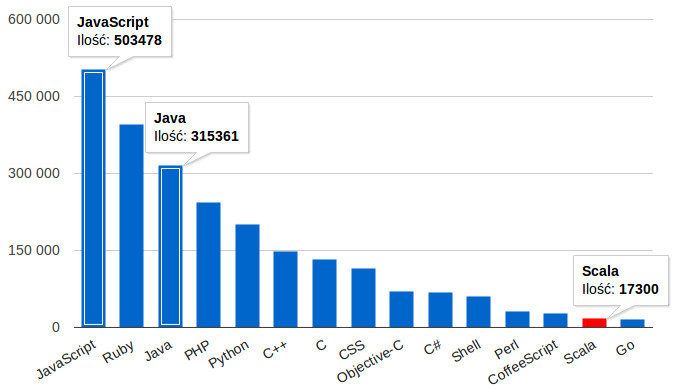
\includegraphics[width=.95\hsize]{fig/top_github_languages_2013}
\caption{Ilość repozytoriów dla poszczegónych języków na platformie GitHub w roku 2013 \label{RYS.1}}
\source{GitHub Archive (www.githubarchive.org)}
\end{figure}

Powyższy wykres przedstawia pierwszych 15 języków, wśród których Scala uplasowała się na miejscu 14. Różnica w liczbie repozytoriów między Scalą, a Javą będącą na trzecim miejscu jest znaczna. Nie ma wątpliwości, że Java swoją wysoką pozycje zawdzięcza wieloletniej obecności na rynku, a także wkładowi jaki do świata technologii informacyjnych wniosła maszyna wirtualna JVM. Na popularność JavaScript'u, czy Ruby'ego częściowo miało wpływ pojawienie się w ostatniej dekadzie narzędzi takich jak \textit{Ruby on Rails}, \textit{node.js}, \textit{AngularJS} i wielu innych. 

Jednak jak pokazuje przykład Ruby'ego i JavaScriptu, jednym z elementów wpływających na popularność jest aktywne środowisko programistów zgromadzonych wokół danego języka. Niejednokrotnie, taka grupa osób przekonana o zaletach swojego ulubionego języka jest w stanie wytworzyć alternatywne sposoby jego promocji. Potwierdzeniem tego może być zespół programistów zgromadzonych wokół platformy \textit{CodeSchool}\footnote{www.codeschool.com}. Opracowali oni szereg prostych kursów związanych głownie z JavaScript'em i Ruby'm w trakcie, których uczestnik rozwiązuje proste zadania programistyczne. 

Żadne z obecnych rozwiązań -- szczególnie dla Scali -- nie posiada jednak możliwości tworzenia własnych zadań dla zamkniętych grup uczestników. Wierzę, że system, który daje sposobność definiowania własnych kursów dla języka Scala może znacząco zwiększyć jej popularność. Implementacja takiego systemu w szkołach i uczelniach mogłaby przynieść również inne korzyści, jak na przykład wzrost zainteresowania programowaniem, czy podniesieniem umiejętności przyszłych programistów przy jednoczesnym zmniejszeniu nakładu pracy prowadzących zajęcia.

\section{Język Scala}

Pomysłodawcą i głównym twórcą Scali jest niemiecki profesor Martin Odersky. Nazwa języka ma na celu sugerować, że jest on skalowalny\footnote{ang: Scalable language}. Scala rośnie wraz z potrzebami jej użytkowników. Cały czas powstają kolejne narzędzia i biblioteki mające uprościć pracę z nią, czy też dodać do niej coś nowego. 

Jedną z ciekawostek wprawdzonych przez Scalę jest interpreter o nazwie REPL\footnote{ang: Read-Evaluate-Print Loop}. Interaktywny interpreter dla języka statycznie typowanego to przecież połączenie dwóch odrębnych światów. REPL potrafi między innymi podpowiedzieć ścieżki do paczek i klas, czy możliwe do wywołania metody na danych bytach po wciśnięciu klawisza tabulacji. Jest do doskonałe narzędzie do sprawdzania małych fragmentów kodu.

Scala łączy ze sobą paradygmat programowania obiektowego oraz funkcyjnego. Umożliwia wykorzystanie najlepszych cech tych dwóch podejść w projektowaniu nowych systemów. Sprawdzi się zatem doskonale zarówno podczas pisania małych jak i dużych projektów.

W przypadku tych pierwszych, programowanie funkcyjne w większości jest dobrym wyborem, gdyż posiadany jest stały zbiór rzeczy. Wraz z ewolucją kodu, dodawane są głównie nowe operacje na istniejących bytach. Dokonuje się tego poprzez dodawanie nowych funkcji, które wykonują obliczenia opierając się na istniejących typach danych. 

Przeciwieństwem jest programowanie obiektowe, które jest dobrym wyborem kiedy dysponujemy stałym zestawem operacji na rzeczach, a w czasie ewolucji kodu dodawane są nowe byty jak klasy. Gdy istnieje, więc potrzeba zaimplementowania dużego systemu, który będzie wymagać rozwijania i dostosowywania do nowych potrzeb, paradygmat programowania obiektowego sprawdzi się lepiej.

\subsection{Aspekt obiektowy}

Scala jest całkowicie zorientowana obiektowo. Inaczej niż w wielu językach obiektowych, nie posiadamy tutaj wartości, które nie są obiektami jak np. typy prymitywne w Javie. Każda wartość jest obiektem, a każda operacja jest wywołaniem metody. 

Ponadto zezwala ona na zdefiniowanie metod o nazwie przypominającej operator. Przykładem może być metoda \texttt{:::} konkatenująca listy, czy metoda \texttt{!} w klasie \texttt{Actor}. Tworzenie nowych obiektów w Scali jest również bardzo elastyczne. Komponent zwany cechą (ang. trait) jest czymś, czym dla Javy są interfejsy. Jednak w porównaniu do interfejsów, cechy mogą zawierać implementacje pól oraz metod. 

Dzięki cechom, Scala idzie także o krok dalej w kwestii kreowania obiektów. Dobrym przykładem tego może być wielokrotne dziedziczenie, które można osiągnąć w poniższy sposób.

\inputminted[fontsize=\small]{scala}{code/multipleInheritance.scala}

Należy w uzupełnieniu do powyższego przykładu wspomnieć jak Scala interpretuje konstrukcję \texttt{super}. Otóż będzie ona wywołana zawsze w tym miejscu, w którym się pojawia. Odpowiada za to proces linearyzacji. Podczas tworzenia instancji danej klasy, Scala układa wszystkie klasy i cechy, po których ta klasa dziedziczy w liniowej kolejności. Dowodem niech będzie wywołanie metody \texttt{get} dla wcześniej pokazanego kodu w interpreterze Scali.

\begin{minted}[fontsize=\small]{scala}
scala> new MyNumber(5).get
res0: Int = 9
\end{minted}

Liczba 5 została tutaj najpierw zmniejszona o 1, następnie pomnożona przez 2 i ostatecznie dopiero na końcu powiększona o 1. Zmieniając jednak kolejność cech wmieszanych w klasę \texttt{MyNumber} osiągniemy inny wynik.

\begin{minted}[fontsize=\small]{scala}
scala> class MyNumber(number: Int) extends Number(number: Int) 
         with Incrementing with Doubling with Decrementing
defined class MyNumber

scala> new MyNumber(5).get
res1: Int = 11
\end{minted}

Liczba 5 została tutaj najpierw zwiększona o 1, w następnym kroku pomnożona przez 2, by wynik tego działania pomniejszyć o 1. Metoda \texttt{get} zwraca w tym przypadku 11, wykonując działania w odwrotnej kolejności niż przedtem.

Warto wspomnieć również o klasach poprzedzonych modyfikatorem \texttt{case}. Kompilator Scali dodaje kilka udogodnień dla takich bytów. 

Pierwszym z nich jest dodanie metody fabrycznej o nazwie takiej jak klasa. Oznacza to, że tworząc nowy obiekt takiego typu nie jest obowiązkowym podawanie instrukcji \texttt{new}. 

\begin{minted}[fontsize=\small]{scala}
scala> case class MyNumber(number: Int)
defined class MyNumber

scala> val mn = MyNumber(5)
mn: MyNumber = MyNumber(5)
\end{minted}

Drugim ułatwieniem jest fakt, że wszystkie argumenty automatycznie stają się polami danej klasy. Dla porównania, w klasach bez modyfikatora \texttt{case} nie można się odwołać do nich z zewnątrz, a żeby parametr był rozpatrywany jako pole wymaganym jest podanie prefiksu \texttt{val}.

\begin{minted}[fontsize=\small]{scala}
scala> class Cat(name: String)
defined class Cat

scala> case class Dog(name: String)
defined class Dog

scala> new Cat("Nazir").name
<console>:9: error: value name is not a member of Cat
              new Cat("Nazir").name
scala> Dog("Luna").name
res7: String = Luna           
\end{minted}

Trzecim udogodnieniem są implementacje metod \texttt{toString} oraz \texttt{equals}. Pierwsza z nich zwróci ciąg znaków w postaci nazwy klasy wraz z aktualnymi wartościami pól. Druga potrafi porównać całe drzewo klas i w sposób rekursywny wszystkie argumenty obiektów. Ponieważ w Scali operator \texttt{==} zawsze odwołuje się do metody \texttt{equals} to tego typu klasy automatycznie porównywane są w sposób strukturalny.    

Komponentom z modyfikatorem \texttt{case} kompilator dodaje jeszcze jedną wygodną metodę -- \texttt{copy}. Zwraca ona kopię obiektu w postaci nowej instancji klasy, gdzie różne są wartości niektórych pól. Korzysta ona z parametrów opisanych nazwami. Gdy nie zostaje podana nazwa danego pola to zwracana jest stara, nie zmodyfikowana wartość. 

\begin{minted}[fontsize=\small]{scala}
scala> val d = Dog("Luna")
d: Dog = Dog(Luna)

scala> d.copy(name = "Azor")
res1: Dog = Dog(Azor)
\end{minted}

Jedynym kosztem użycia modyfikatora \texttt{case} przed definicją klasy jest fakt, że obiekt staną się nieco większe. Dzieje się tak z powodu dodatkowych metod. Największą zaletą jednak jest możliwość użycia takich klas w mechanizmie dopasowywania wzorca opisanego w późniejszej części tego rozdziału.

\subsection{Aspekt funkcyjny}

Jak wyjaśnia Martin Odersky, ,,programowanie funkcyjne w głównej mierze opiera się na dwóch założeniach'' \cite[s.57]{Odersky:2010:PIS}. Wskazane jest aby funkcje były wartościami podstawowymi, a operacje wykonywane w czasie działania programu powinny zwracać wartości do nowych zmiennych niż modyfikować obecne. Obie te koncepcje są oczywiście obecne w Scali. 

Możemy przekazywać funkcję jako argument do innej funkcji, po to aby w odpowiedzi otrzymać jeszcze inną funkcję. Możliwe jest także definiowanie funkcji wewnątrz innych funkcji. Funkcje mogą posiadać nazwe lub być też anonimowe. Żadna z wymienionych opcji nie jest możliwa chociażby w Javie, aż do wersji 8, która to dopiero pozwala na użycie funkcji anonimowych. Wszystkie te warianty mają bezpośredni wpływ na skalowalność programów.

Inspiracja do poniższego przykładu pochodzi z książki ,,Scala by Example'' profesora Martina Oderskiego \cite[s. 22]{Odersky:2014:SBE}. Korzystając z interpretera pokazuje on w prosty sposób jak może wyglądać praca z funkcjami w Scali. Zdefiniowane zostały dwie funkcje -- \texttt{sum} oraz \texttt{sumSquares}.

\begin{minted}[fontsize=\small]{scala}
scala> def sum(f: Int => Int, a: Int, b: Int): Int = f(a) + f(b)
sum: (f: Int => Int, a: Int, b: Int)Int

scala> def sumSquares(a: Int, b: Int): Int = sum((x: Int) => x * x, a, b)
sumSquares: (a: Int, b: Int)Int

scala> sumSquares(3, 4)
res0: Int = 25
\end{minted}

Pierwszym parametrem \texttt{sum} jest funkcja (f), która za argumenty przyjmuje liczby całkowite. Zobligowana jest także do zwrócenia wartości tego typu. W ciele funkcji \texttt{sum} widać, że na pozostałych dwóch argumentach (a i b) wywołana zostaje funkcja \texttt{f}. Dodane do siebie zostają bowiem wartości \texttt{f(a)} i \texttt{f(b)}. Zdefiniowano, więc funkcję posiadającą w liście argumentów inną funkcję. W ciele funkcji \texttt{sumSquares}, \texttt{sum} zostaje wywołana poprzez podanie jako pierwszego argumentu funkcji anonimowej.

Autorzy ,,Programming in Scala'' posłużyli się doskonałym przykładem wyjaśniającym drugie założenie. \cite[s.57]{Odersky:2010:PIS} Otóż należy rozpatrzeć implementacje ciągu znaków w języku Ruby i Java. W Ruby'm, ciag znaków jest niczym innym jak tablicą znaków. Możemy zatem każdy znak w danym ciągu podmieniać wewnątrz tego samego obiektu. W Javie, typ \texttt{String} jest ciągiem znaków w sensie matematycznym. Aby wykonać podobną operację konieczne jest wywołanie metody \texttt{replace}, która zwraca zupełnie nowy obiekt.

Prawdziwy język funkcyjny wymusza na programiście, aby ten korzystał z niezmiennych danych. Scala daje możliwość wyboru, ale jednocześnie zachęca do unikania imperatywnych konstrukcji. Pracując z funkcyjnym językiem programowania nie unikniemy także niezmiennych struktur danych. Scala posiada również własny zestaw niezmiennych typów jak na przykład listy, czy zbiory. Idea wykonywania operacji na nich jest zbliżona do koncepcji niezmiennych wartości.

\begin{minted}[fontsize=\small]{scala}
scala> val list = List(1,2,3)
list: List[Int] = List(1, 2, 3)

scala> list :+ 4
res0: List[Int] = List(1, 2, 3, 4)
\end{minted}

Dla przykładowej trzyelementowej listy liczb całkowitych, wykonując operację dodawania nowego elementu do niej w wyniku zwrócony zostaje nowy obiekt reprezentujący listę czteroelementową. W imperatywnym języku programowania, taka operacja zmodyfikowałaby wcześniej utworzony obiekt. 

\subsection{Pozostałe cechy}

Oprócz łączenia technik programowania obiektowego i funkcyjnego, Scale definują cechy takie jak kompatybilność z JVM, zwięzłość, wysoki poziom abstrakcji i statyczne typowanie. 

\subsubsection{Kompatybilność}

Wydajność programów napisanych w Scali jest porównywalna z odpowiednikami napisanymi w Javie. Programy te bowiem kompilują się do pseudokodu wirtualnej maszyny Javy. Ponadto są w stanie bez przeszkód wywoływać metody klas Javy, korzystać z ich pól, a nawet przystosowywać własne komponenty poprzez dziedziczenie z klas Javy, czy implementację interfejsów. Każdy z tych wariantów jest wykonywany przez programistę w sposób naturalny, gdyż nie wymaga to użycia żadnej dodatkowej składni. Jak się okaże w później, system będący głównym tematem pracy również korzysta z dobrodziejstw owej kompatybilności. Korzysta on z oficjalnego klienta dla systemu kolejkowania wiadomości \emph{RabbitMQ} dla języka Java.

Scala korzysta w pełni z typów Javy. Typ \texttt{Int} w Scali reprezentuje prymitywne liczby całkowite \texttt{int} z Javy. Podobnie ma się sytuacja z \texttt{Float}, \texttt{Double}, \texttt{Long}, czy \texttt{Boolean}. Ponadto typy zostają ,,opakowowane'' w taki sposób, aby wywołania metod związanych z nimi były bardziej przejrzyste. W efekcie tego, dla przykładu zamiast \texttt{Double.parseDouble("12.0")} wystarczy napisać \texttt{"12.0".toDouble}.

\subsubsection{Zwięzłość}

Scala zachęca do zwięzłego i czytelnego stylu programowania. Porównując kod Scali i Javy ze sobą, niejednokrotnie okazuje się, że kod Scali jest krótszy o ponad połowę. Taka forma pozwala na jego większe zrozumienie, łatwiejsze utrzymanie przy jednoczesnym mniejszym wysiłku. Wynika to głównie ze składni języka, gdzie między innymi średniki na końcu instrukcji są opcjonalne. Pisząc funkcję, w wielu miejscach można pominąć klamry otwierające i zamykajace dany blok kodu. Jednak najbardziej tą różnice pokazuje porównanie tworzenia klas z konstruktorem.

\inputminted[fontsize=\small,label=Person.java,frame=single,framerule=0pt,framesep=2pt]{java}{code/person.java}

\inputminted[fontsize=\small,label=Person.scala,frame=single,framerule=0pt,framesep=2pt]{scala}{code/person.scala}

\subsubsection{Wysoki poziom}

Język wysokiego poziomu to taki, który pozwala człowiekowi szybko zrozumieć kod programu. Scala jest typem takiego języka. Programista może przy pomocy dostępnych mu komponentów takich jak cechy, czy literałów funkcyjnych w dużo lepszy sposób zarządzać poziomem skomplikowania kodu. Znów warto w tym momencie porównać ze sobą Jave i Scalę. Niech problemem do rozwiązania, będzie znalezienie wszystkich liczb parzystych z przedziału od 1 do 10. W Scali to zagadnienie można rozwiązać w jednej linijce.

\mint[fontsize=\small]{scala}/val evenNumbers = (1).to(10).toList.filter(_ % 2 == 0)/

Natomiast w Javie, ten sam problem wymaga od programisty odpowiednio więcej pracy.

\begin{minted}[fontsize=\small]{java}
List<Integer> numbers = Arrays.asList(1, 2, 3, 4, 5, 6, 7, 8, 9, 10);
List<Integer> evenNumbers = new ArrayList<Integer>();
for(Integer number: numbers){
    if(number % 2 == 0){
        evenNumbers.add(number);
    }
}
\end{minted}

W drugim rozwiązaniu potrzebne były dwie listy oraz pętla iterująca po wszystkich liczbach z danego zakresu. W Scali wystarczy użyć odpowiedniej metody (\texttt{filter}), która jako argument przyjmuje predykat \texttt{\_ \% 2 == 0 }, będący przykładem literału funkcyjnego. Jest to jednoargumentowa funkcja sprawdzająca dzielenie modulo.

Wyraźnie widać, że rozwiązanie przedstawione w Scali jest krótsze. Z własnych doświadczeń wiem, że zbyt skomplikowany kod potrafi w pracy programisty utrudnić pracę do tego stopnia, że dochodzi do potrzeby przepisania jakiegoś fragmentu systemu. Zawsze oznacza to dodatkowy koszt, w postaci czasu, pieniędzy czy zasobów ludzkich. Scala posiada wszystko, by przy relatywnie niedużym wysiłku sprawić, aby skomplikowana logika biznesowa stała się zrozumiała i czytelna.

\subsubsection{Typowanie statyczne}

Scala jest językiem statycznie typowanym. Podstawowe zalety jakie niesie to ze sobą to możliwość wykrycia błędów związnych z typowaniem na etapie kompilacji, bezpieczny refaktoring i powstanie bardziej szczegółowej dokumentacji. 

Jednym z zarzutów stawianych językom z typowaniem statycznym jest to, że są bardziej ,,rozgadane''. Przyczyny można szukać w konieczności deklarowania typów zmiennych, czy wartości wynikowych funkcji. W Scali obecna jest inferencja typów -- mechanizm potrafiący wywnioskować typ dla danej wartości. Niech przykładem będzie zmienna \texttt{numbers} z wcześniej przedstawionego fragmentu kodu Javy. W Scali nie musimy (choć możemy) określić, że zmienna \texttt{numbers} jest listą liczb całkowitych. Poniżej kontrprzykład.

\mint[fontsize=\small]{scala}/val numbers = List(1, 2, 3, 4, 5, 6, 7, 8, 9, 10)/

Należy jednak pamiętać, że funkcje rekursywne muszą mieć zawsze określony typ wynikowy, aby nie doszło do błędu kompilacji. Rozpatrzmy funkcję obliczającą liczbę Fibonacciego.

\begin{minted}[fontsize=\small]{scala}
def fib(n: Int): Int = n match {
  case 0 => n
  case 1 => n
  case _ => fib(n - 1) + fib(n - 2)
}
\end{minted}

Gdyby nie określono tutaj typu wynikowego funkcji, to kompilator nie wiedziałby o jakiej operacji ,,+'' myślał programista, tzn. dla jakiego typu. Przy okazji udało się tutaj zaprezentować dopasowywanie wzorca \footnote{ang: Pattern matching}.

Technika ta pozwala w czytelny dla człowieka sposób określić jakie powinny być następne instrukcje programu w zależności od zmiennej. Dopasowywać można nie tylko do konkretnej wartości, ale przede wszystkim typu. Ma to znaczenie w przypadku, gdy porównujemy ze sobą na przykład typy dziedziczące po wspólnej klasie w hierarchii.

\begin{minted}[fontsize=\small]{scala}
case class Animal
case class Cat extends Animal
case class Dog extends Animal

def say(a: Animal) = a match {
 case a: Cat => println("Meow!")
 case a: Dog => println("Woof!")
 case _ => println("Animal")
}
\end{minted}

Znak podkreślnika można traktować jak instrukcję \texttt{else}.

\section{Środki do osiągnięcia celu}

Do weryfikacji poprawności nadesłanego przez użytkownika rozwiązania, niezbędnym jest posłużenie się narzędziami związanymi z mechanizmem testów jednostkowych. Testy te muszą być uruchamiane automatycznie po przesłaniu rozwiązania. W osiągnięciu takiego celu pomogą narzędzia takie jak \textit{Simple Build Tool} wraz ze \textit{ScalaTest} i \textit{ScalaCheck}. Połączenie ich ze sobą umożliwi powstanie bardzo elastycznego procesu tworzenia zadań. 

Poniżej znajduje się krótkie przedstawienie tych narzędzi wraz z uzasadnieniem ich użycia. 

\subsection{Simple Build Tool}

SBT jest narzędziem, które tworzy stabilną platformę do rozwijania aplikacji. Domyślnie udostępnia programiście listę komend, z których może on korzystać. Dla przykładu komendy te mogą służyć przeładowaniu definicji projektu, uruchomieniu testów, czy uruchomieniu interpretera Scali z gotowymi do użycia klasami z danego projektu. Zdecydowanie sprzyjają one zwiększeniu produktywności programisty poprzez automatyzację pewnych działań.

Jednak warto przyjrzeć się bliżej dlaczego w ogóle warto korzystać z narzędzi budujących aplikację\footnote{ang: Build tool} oraz w jaki sposób wykorzystanie SBT jest kluczowe dla systemu weryfikującego kod. 

Autorzy książki ,,SBT in Action'' już na początku podają prosty przykład w jaki sposób tego typu narzędzia zwiększają produktywność nawet całego zespołu programistów. Wspominają o tym jak kilka lat temu w jednym z zespołów odbywało się ,,automatyczne'' budowanie projektu. ,,To było 10 lub 12 okienek z plikami .batch, które budowały i instalowały aplikację. Kompilowały pliki Java, budowały aplikacje internetową i instalowały ją na serwerze. Zajmowało to od 1,5 do 2 godzin -- to była lekcja jak nie automatyzować''.\cite[s.1]{Suereth:2014:SIA} Jak twierdzą, po przepisaniu skryptu i użyciu narzędzia \emph{Apache Ant} czas ten zmalał do około 8 minut.

Czas zatem odpowiedź na pytanie -- dlaczego SBT? Kilka najważniejszych powodów to:
\begin{itemize}
\item krótki czas kompilacji -- kompilowane są tylko ostatnio zmodyfikowane pliki
\item wbudowane polecenia uruchamiające testy, kompilujące pliki źródłowe oraz pakujące poszczególne typy plików do archiwum .jar
\item możliwość sprawdzania klas projektu przy użyciu Scala REPL
\item prostota dodawania własnych poleceń mogących wykonywać specyficzne dla projektu zadania   
\end{itemize}

Dla mojego systemu to właśnie ostatni punkt ma szczególne znaczenie. System ten będzie udostępniać projekt stworzony przy użyciu SBT, na którym docelowo będą uruchamiane testy. Projekt SBT może być potraktowany w całości lub tylko częściowo jako zadanie do rozwiązania. Aby system mógł sprawdzić rozwiązanie, użytkownik musi je w jakiś sposób przesłać. Dzięki SBT, w sposób wygodny może odbyć się to poprzez napisaną przeze mnie komendzie \texttt{sendSolution}, która jako argumenty bierze adres e-mail i hasło użytkownika. Pomysł na takie rozwiązanie został zaczerpnięty z kursów edukacyjnych organizowanych przez profesora Oderskiego na platformie \textit{Coursera}\footnote{\url{https://www.coursera.org/}}. Jest ono wygodne, ponieważ polecenie jest wywoływane z poziomu projektu, a także pozwala zaoszczędzić czas, który użytkownik normalnie spędziłby na przykład na pakowaniu plików do archiwum, logowaniu się na pocztę elektroniczną i tworzeniu wiadomości z załącznikiem.

\subsection{ScalaTest}

\label{scalaTestSrodek} 

ScalaTest to popularne narzędzie do testowania programów, którego autorem jest programista Bill Venners. Podobnie jak w przypadku języka Scala, jednym z założeń ScalaTestu jest skalowalność. Dzięki temu obecna wersja\footnote{W chwili pisania pracy -- najnowsza dostępna wersja ScalaTest to 2.1.6} to nie jedno narzędzie, lecz cały zestaw. Jest on zintegrowany z listą instrumentów związanych z pisaniem testów dla Scali i Javy. Instalując więc ScalaTest w swoim projekcie, możemy korzystać również między innymi z \textit{JUnit, JMock, EasyMock, Mockito, ScalaMock}, czy \textit{Selenium}. Ponadto ScalaTest z łatwością współpracuje z najpopularniejszymi zintegrowanymi środowiskami programistycznymi -- \textit{Eclipse}, \textit{IntelliJ} oraz \textit{NetBeans}.

Szczególnie ważnym argumentem przemawiającym za ScalaTest jest możliwość wybrania przez użytkownika stylu specyfikacji. Z punktu widzenia mojego systemu, ta sposobność wyboru wraz ze wspominaną wcześniej szeroką gamą narzędzi gwarantuje dużą uniwersalność dla użytkowników układających zadania. Chociaż szczegółowa charakterystyka systemu znajduje się w późniejszej części pracy to już teraz można wyobrazić sobie sytuację, w której z systemu korzysta kilka osób odpowiedzialnych za układanie projektów-zadań. Każda z nich może posiadać nie tylko różne doświadczenia w Scali, ale także różne preferencje w kwestii przywoływanych narzędzi, czy pisania specyfikacji. 

Podobnie sytuacja ma się w stosunku do użytkowników rozwiązujących zadania. Wyobrażam sobie ich jako przyszłych programistów, a zatem dobrą praktyką byłoby, aby przed wysłaniem rozwiązania potrafili je przetestować, przy okazji poznając różne techniki testowania w Scali. 

\subsection{ScalaCheck}

\label{scalaCheckSrodek}

Biblioteka \emph{QuickCheck} dla języka Haskell, była inspiracją, dzięki której powstał ScalaCheck. Jego zadaniem jest w pełni zautomatyzować testy w taki sposób, aby nie było potrzeby wprowadzania danych testowych do sprawdzanych metod własnoręcznie. Generuje pseudolosowe dane jako argumenty, co pozwala zaoszczędzić czas, który normalnie programista spędza chociażby na wymyślaniu danych testowych. Ponadto sprawia, że kod jest bardziej odporny na błędy ponieważ, zwiększa zakres sprawdzanych wartości, które program może otrzymać w trakcie działania.

Powyższy fakt oraz to, że ScalaCheck integruje się z ScalaTest może zagwarantować wysoką jakość podczas weryfikacji kodu w rozwiązaniach użytkowników. Użytkownik odpowiedzialny za tworzenie projektów-zadań poprzez stosowanie reguł ScalaCheck powinien być w stanie wytworzyć kompletny zestaw testów. Dzięki nim system będzie potrafił w sposób dużo bardziej rzetelny wystawić noty za rozwiązanie.
      
\chapter{Testowanie kodu napisanego w Scali}      

Projekty powstające niezależnie w jakim języku programowania muszą być przetestowane. Nie inaczej jest, gdy programy te napisane są w Scali. Podczas wszystkich lat rozwoju branży IT pojawiło się wiele metodologii, narzędzi oraz rodzajów testów. Wyróżnić można testy akceptacyjne, funkcjonalne, jednostkowe, czy integracji. Z punktu widzenia aplikacji będącej tematem pracy to testy jednostkowe są najważniejszym elementem gwarantującym jej poprawne działanie.       
      
\section{Mechanizm testów jednostkowych}

Czym jest test jednostkowy? Andy Hunt i Dave Thomas napisali kiedyś, że ,,test jednostkowy to kawałek kodu napisanego przez programistę, który sprawdza bardzo małą, specificzną część funkcjonalności testowanego kodu.''\cite[s.3]{Hunt:2003:PUT} Im, większe pokrycie kodu testami, tym większa pewność, że program spełni stawiane przed nim wymagania bez efektów ubocznych. Roy Osherove natomiast określił cechy dobrego testu jednostkowego\cite[s. 6]{Osherove:2009:TAOUT} 

\begin{itemize}
\item Szybki, automatyczny i powtarzalny
\item Łatwy do zaimplementowania
\item Napisany raz, powinien pozostać w takim stanie w przyszłości
\item Każdy powinien być w stanie go uruchomić
\item Uruchamiany ,,wciśnięciem guzika'' 
\end{itemize}

Testy jednostkowe są esencją systemu weryfikującego kod. To od nich w dużej mierze zależna jest ocena jakości kodu. Muszą one, więc sprawdzać nie tylko poprawność efektów dokonywanych przez funkcje i metody, ale także odporność na błędy.  

Obecnie istnieje wiele narzędzi zajmujących się zagadnieniem testów jednostkowych w Scali. Najbardziej popularne z nich to \emph{ScalaTest}, \emph{JUnit} i \emph{Specs2}.

Pierwszy z nich po krótce przedstawiłem podrozdziale \ref{scalaTestSrodek} w kontekście zastosowania do systemu weryfikującego kod. W tym rozdziale ScalaTest zostanie omówiony bardziej szczegółowo. 

JUnit natomiast to narzędzie znane wszystkim programistom Javy. Kompatybilność z wirtualną maszyną JVM powoduje, że może bez przeszkód mieć zastosowanie również w Scalowych projektach. Warto przypomnieć, że narzędzie to integruje się z ScalaTest. 

O ostatnim z wymienionych -- Specs2 -- można myśleć jak o konkurencji ScalaTestu. Narzędzie to może również działać z SBT. Posiada inny zestaw instrukcji dokonujących porównań oraz sposób konstruowania testów. To co szczególnie wyróżnia Specs2 to fakt, że testy są uruchamiane równolegle, każdy w osobnym wątku.
      
\section{ScalaTest}

Testy w ScalaTest tworzy się, poprzez napisanie klasy testującej dziedziczącej po jednej z wybranych cech determinujących styl testów. Końcowym efektem są specyfikacje będące ważnym elementem w metodologii \emph{Behavior-driven development} (BDD). Polega ona na definiowaniu testów w sposób opisowy, tak jakby fragmenty testowanego kodu były elementami pewnych historii. Schemat, w który wpisują się wszystkie poprawnie opisane testy wygląda następująco: ,,Posiadając.., jeśli.., wtedy..''\footnote{ang: Given, When, Then}. Słowo ,,test'' natomiast zastąpione zostaje słowem ,,zachowanie'' (ang: behavior). Ideą BDD jest, aby poprzez tak skonstruowane specyfikacje zespół programistów potrafił w pełni zrozumieć potrzeby i intencje klienta. Dostarczone oprogramowanie ma wtedy spełniać wszystkie założenia i wymagać mniej poprawek po wdrożeniu produkcyjnym.

ScalaTest poza stylem specyfikacji daje programiście wybrać, także detale takie jak sposób weryfikacji rezultatów w teście. Istnieją klasyczne asercje poprzedzane instrukcją \texttt{assert}, ale także weryfikatory, które zasługują na szczególną uwagę. Są to specjalne asercje pozwalające czytać test, jak zwykłe zdanie. W przypadku nie powodzenia testu, rzucany jest wyjątek \texttt{TestFailedException}. ScalaTest przechwytuje je i zaznacza dany test jako nie zaliczony.

\subsection{Style specyfikacji}

ScalaTest pozwala programiście wybrać jeden z wielu stylów dla swoich specyfikacji. Twórcy zaznaczają jednak, aby podczas rozwijania projektu przez dany zespół nie doszło do sytuacji, w której każdy programista pisałby w inny sposób. Zalecanym jest, aby testy jednostkowe powstawały przy użyciu jednego głównego stylu, a na przykład testy integracji, czy akceptacyjne w innym. Ma to pomóc poszczególnym członkom zespołu ,,przełączać się'' pomiędzy testami niskiego i wysokiego poziomu.

W podrozdziale \ref{scalaTestSrodek} można było przeczytać jak tą elastyczność ScalaTestu można wykorzystać w systemie sprawdzającym kod Scali. Poszczególne style specyfikacji różnią się jedynie instrukcjami deklarującymi testy. Pozostałe rzeczy takie jak asercje, instrukcje dopasowywania (ang: Matchers) określane przeze mnie weryfikatorami są wykorzystywane w ten sam sposób.

Poniżej znajduje się zestawienie kilku wybranych styli oferowanych przez ScalaTest. Przykłady pochodzą z oficjalnej strony projektu\footnote{\url{http://www.scalatest.org/user_guide/selecting_a_style}}.

\subsubsection{FunSuite}

Charakteryzuje się opisowymi nazwami testów i jest najprostszym ze wszystkich styli, które oferuje ScalaTest. Testy deklarujemy poprzez instrukcję \texttt{test}, jako argument podając opis testu.

\inputminted[fontsize=\small]{scala}{code/FunSuite.scala}
 
\subsubsection{FlatSpec}

Jest pierwszym przystankiem dla programistów, którzy zaczynają swoją przygodę z BDD. Nazwy testów tworzy się w stylu charakterystycznym dla specyfikacji, tzn. używając słów takich jak \texttt{should}, \texttt{must}.

\inputminted[fontsize=\small]{scala}{code/FlatSpec.scala}

\subsubsection{FunSpec}

Doświadczeni programiści Rubiego próbujący swoich sił w Scali prawdopodobnie wybiorą ten styl. Przypomina on bardzo \emph{RSpec} -- popularne narzędzie testowania kodu Rubiego. Testy można tutaj konstruować głównie przy pomocy \texttt{describe} oraz \texttt{it}. Instrukcja \texttt{describe} pozwala na zagnieżdzanie i grupowanie testów według danego ,,zachowania'' testowanych fragmentów kodu. Jest to dobry wybór dla zespołów pracujących w BDD.

\inputminted[fontsize=\small]{scala}{code/FunSpec.scala}

\subsubsection{WordSpec}

Sposób konstrukcji testów jest bardzo ścisły i przypomina konkurencyjny \emph{Specs2}. Gdyby zatem w projekcie doszło do potrzeby przejścia ze \emph{Specs2} na ScalaTest, to ten styl staje się naturalnym wyborem. Słowami kluczowymi są tutaj \texttt{when} oraz \texttt{should}.

\inputminted[fontsize=\small]{scala}{code/WordSpec.scala}

\subsubsection{FreeSpec}

Wskazany dla doświadczonych programistów piszących specyfikacje, ponieważ nie istnieją żadne wytyczne jak powinien powstawać test przy użyciu tego stylu. Testy można w dowolny sposób zagnieżdzać i nazywać.

\inputminted[fontsize=\small]{scala}{code/FreeSpec.scala}

% Pominięte style
%\subsubsection{Spec}
%Zalecany przez twórców do dużych projektów, gdzie czas budowania i kompilacji może być znaczny. Konstruując test definuje się go jako metodę zawierającą jeden literał funkcyjny.
%\inputminted[fontsize=\small]{scala}{code/Spec.scala}
%\subsubsection{PropSpec}
%Testy w tym stylu skupiają się na własnościach testowanych metod i funkcji. Specyfikacje tworzone przu użyciu PropSpec przypominają na pierwszy rzut oka FunSuite z tą różnicą, że główną instrukcją %definiującą test \emph{property}.
%\inputminted[fontsize=\small]{scala}{code/PropSpec.scala}
%\subsubsection{FeatureSpec}
%Jest przeznaczony dla testów akceptacyjnych. Szeroki zestaw instrukcji takich jak \emph{info}, \emph{scenario}, \emph{feature} oraz \emph{Given}, \emph{When} \emph{Then} pozwala zrozumieć dany test %nawet osobom nie zajmującym się oprogramowaniem danego projektu. Mogą one w ten sposób określić, czy program wykonuje założone cele i przyspieszyć komunikację między nimi, a programistami.
%\inputminted[fontsize=\small]{scala}{code/FeatureSpec.scala}

\subsection{Weryfikatory}

\label{weryfikatory}

Bez względu na to jaki wybierzemy styl dla specyfikacji to rezultaty testowanych metod i funkcji muszą być w jakiś sposób sprawdzone. ScalaTest dostarcza specjalny język dziedzinowy dla asercji. Po dodaniu do klasy specyfikacji cechy \texttt{Matchers} otrzymujemy weryfikatory. Dzięki nim można przystąpić do tworzenia czytelnych asercji. Poniżej przykład.

\begin{minted}[fontsize=\small]{scala}
val list = List(2, 4, 5)
list.size should be (3)
list.size should equal(3)
list.size should be < (10)
list.size should not be >= (20)
list should contain (4)
\end{minted}

Wartość, która jest oczekiwana od testowanej metody dopasowana została do jej faktycznego wyniku przy użyciu słowa \texttt{should}. Całość można przeczytać płynnie jak zdanie w języku angielskim. 
Chcąc sprawdzić, czy zwrócona wartość równa się temu czemu powinna należy użyć instrukcji \texttt{equal} lub \texttt{be}. Drugą z nich można łączyć dodatkowo ze znakami większości i mniejszości. Pod koniec tego przykładu zaprezentowałem również w jak prosty sposób można sprawdzić, czy lista zawiera dany element.

Istnieje wiele wariantów testowania ciągów znaków. Można sprawdzić ,czy dany ciąg znaków zawiera inny lub zaczyna się, czy kończy w określony sposób. Oczywiście w przypadku bardziej skomplikowanych wymogów, nie ma przeszkód aby dopasować i porównać wynik przy pomocy wyrażeń regularnych.

\begin{minted}[fontsize=\small]{scala}
val sentence = "I love Scala!"
sentence should startWith ("I love")
sentence should not endWith ("Java")
sentence should include ("love")
sentence should endWith regex ("Sca.*!")
sentence should fullyMatch regex ("I.*S.*!+")
\end{minted}

Ponownie dzięki weryfikatorom, osoba czytająca przedstawiony w ten sposób test ma wrażenie, że czyta zwykłe zdanie. Pierwsza asercja sprawdza, czy dany ciąg znaków zaczyna się na ,,I love''. Druga poprzez wstawienie instrukcji \texttt{not} dodaje zaprzeczenie, aby miec pewność, że ciąg znaków nie kończy się słowem ,,Java''. Chcąc dopasować wartość z użyciem wyrażenia regularnego, wystarczy do poznanej już konstrukcji dodać \texttt{regex}. Ostatnia z pokazanych asercji dopasowuje wyrażenie do całego ciągu znaków.

Ciekawą rzeczą jest porównywanie ze sobą liczb zmiennoprzecinkowych. Można określić tolerowany zakres błędu w wyniku działania poprzez postawienie obok siebie znaku dodawania i odejmowania.

\begin{minted}[fontsize=\small]{scala}
(1.5 - 0.5) should be (1.1 +- 0.9)
\end{minted}

Powyższa asercja sprawdza, czy wynik działania tj. 1.0 jest mniejszy niż 1.1 oraz większy od 0.9.

Zweryfikowanie, czy referencje odnoszą się do tych samych obiektów następuje przy użyciu \texttt{theSameInstanceAs}.

\begin{minted}[fontsize=\small]{scala}
val cat1 = new Cat
val cat2 = cat1
val cat3 = new Cat	
cat1 should be theSameInstanceAs (cat2)
cat3 should not be theSameInstanceAs (cat1)
\end{minted}

Instancje \texttt{cat1} oraz \texttt{cat2} odwołują się do tego samego obiektu i jest to zbadane w pierwszej asercji. Natomiast ponownie dodając słowo \texttt{not} uzyskuje się zaprzeczenie.

ScalaTest dostarcza również metody pozwalające łączyć ze sobą asercje w jedną całość. Służą do tego instrukcje \texttt{and}, \texttt{or}. Dla kontrastu, przykład z weryfikatorami w liście można przedstawić w następujący sposób.

\begin{minted}[fontsize=\small]{scala}
list.size should (equal(3) or (be < (10) and (be >= 20)))
\end{minted}

Zyskuje się w ten sposób oszczędność zajętych linii kodu. Należy jednak uważać na składnie. Każda następna asercja musi być zagnieżdzona w kolejną parę nawiasów.

Na zakończenie tej prezentacji weryfikatorów, przykład w jak prosty sposób można przetestować atrybuty obiektów.

\begin{minted}[fontsize=\small]{scala}
class Dog(val name: String)
dog should have (
  'name ("Luna")
)
\end{minted}

Słowem kluczowym jest \texttt{have}, następnie jako symbole podaje się nazwy atrybutów oraz wartość oczekiwaną.

To nie wszystkie weryfikatory, chociaż wierzę, że udało mi się przedstawić te najciekawsze i najważniejsze. ScalaTest daje również możliwość użycia \texttt{MustMatchers}. W praktyce różnica w użyciu tych weryfikatorów sprowadza się do zamiany słowa \texttt{should} na \texttt{must}. Jest to zatem poraz kolejny przykład elastyczności jaką daje to narzędzie.

\mint[fontsize=\small]{scala}/list.size must be (3)/ 

\subsection{Cecha \texttt{GivenWhenThen}}

Dodając do klasy zawierającej zestaw testów cechę \texttt{GivenWhenThen} otrzymujemy kilka użytecznych metod. Ich jedynym zadaniem jest ułatwienie zrozumienia, jak przebiega dana specyfikacja. Są to metody \texttt{Given}, \texttt{When}, \texttt{Then} oraz \texttt{And}. Na przykładzie poniżej znajduje się prosty test sprawdzający dodawanie do bazy danych.

\inputminted[fontsize=\small]{scala}{code/givenWhenThen.scala}

Całość sprowadza się do powstania czytelnej historyjki. ,,Metoda \texttt{create} obiektu \texttt{Group}, powinna zapisać nową grupę w bazie danych. Kiedy grupa jest dodana do bazy danych, wtedy licznik wzrasta i możemy znaleźć tę grupę w bazie danych''. Po uruchomieniu testu, podobny opis otrzymujemy w raporcie końcowym. 

\begin{alltt}
[info] Group.create method
[info] - should save new group in database
[info]   + Given new group instance
[info]   + When Group is being inserted in database 
[info]   + Then collection count increases 
[info]   + And We can find that group in database
\end{alltt}

\subsection{Przechwytywanie wyjątków}

Istnieją dwa sposoby na przetestowanie, czy dany wyjątek został rzucony. Pierwszym z nich jest umieszczenie testowanego fragmentu w blok \texttt{intercept}. Jeśli ten fragment kodu nie rzuci spodziewanego wyjątku to test się nie powiedzie.

\begin{minted}[fontsize=\small]{scala}
import org.scalatest.FunSpec
class SetSpec extends FunSpec {
  describe("A Set") {
    describe("when empty") {
      it("should produce NoSuchElementException when head is invoked") {
        intercept[NoSuchElementException] {
          Set.empty.head
        }
      }
    }
  }
}
\end{minted}

Zdjęcie kolejnego elementu z pustego stosu spowoduje rzucenie wyjątku \texttt{NoSuchElementException}.

Drugi ze sposobów polega na użyciu wcześniej opisywanych weryfikatorów. Testowany fragment kodu należy wstawić w blok \texttt{thrownBy}. Jego przewagą jest to, że rzucony wyjątek można poddać w następnych krokach dodatkowej weryfikacji.

\begin{minted}[fontsize=\small]{scala}
val exc = the [NoSuchElementException] thrownBy { Set.empty.head }
exc.getMessage should include ("empty")
\end{minted}

\subsection{JUnit}

JUnit może być bezpośrednio używany do testowania kodu Scala. Zdecydowanie lepszym rozwiązaniem jest jednak skorzystanie ze sposobności jaką daje ScalaTest w kwestii integracji z tym narzędziem. Zyskuje się w ten sposób dostęp chociażby do weryfikatorów. Aby to zrobić należy klasę z testami rozszerzyć o właściwości cechy \texttt{JUnitSuite}. W ten sposób, możliwe będzie uruchamianie testów z JUnit oraz używanie standardowych asercji. Poznane w podrozdziale \ref{weryfikatory} weryfikatory mogą znaleźć zastosowanie w testach tego rodzaju bez żadnego dodatkowego wysiłku. 

\inputminted[fontsize=\small]{scala}{code/ListSuite.scala}

Ten prosty przykład pokazuje jakie klasy należy zaimportować, aby taka kombinacja dwóch narzędzi przebiegła poprawnie. Klasa \texttt{ListSuite} posiada jeden test oznaczony przez adnotację \texttt{@Test} pochodzącą z narzędzia JUnit. Jego zadaniem jest zweryfikować rozmiar listy. Lista ta zaś zostaje zainicjalizowana przy pomocy innej adnotacji \texttt{@Before}. W metodzie \texttt{checkListSize()} weryfikacja rozmiaru listy przebiega na dwa sposoby. Pierwszy z nich to weryfikator pochodzący ze ScalaTest. Drugi sposób przedstawia standardową asercję pochodzącą z JUnit -- \texttt{assertEquals}.

Jest to także dowód na kompatybilność Scali z klasami Javy i fakt, że dowolna biblioteka stworzona z myślą o Javie, bez przeszkód może być używana w Scalowych programach.

\section{ScalaCheck}

Wspominany już w podrozdziale \ref{scalaCheckSrodek} ScalaCheck zajmuje się automatyzacją testów poprzez generowanie pseudolosowych danych testowych. Składa się z trzech głównych komponentów.
Klasa \texttt{Properties} definuje testy i uruchamia je. Obiekt \texttt{Gen} ma za zadanie generować przykładowe dane i konkretyzować jakiego rodzaju mają one być. Na przykład, jeśli do testowanej metody chcemy przekazać tylko liczby naturalne, przy pomocy \texttt{Gen} można wykluczyć liczby ujemne. Trzecim komponentem jest klasa \texttt{Arbitrary} podejmująca temat specyficznych typów dla programu.

ScalaCheck integruje się również z opisywanym w poprzednim rozdziale ScalaTest.

\subsection{Klasa \texttt{Properties}}

\label{scalaCheck:properties}

Aby rozpoczęć pracę ze ScalaCheck należy zaimportować klasę \texttt{Properties} i rozszerzyć ją przez singleton zawierający zestaw testów. W Scali stworzenie singletonu odbywa się przy pomocy słowa kluczowego \texttt{object}. Najważniejszą i najczęściej używaną metodą jest \texttt{forAll} umieszczona w cesze \texttt{Prop}.

\inputminted[fontsize=\small]{scala}{code/CalcTestBad.scala}

Rozpatrując powyższy przykład można szyko zauważyć, że test nie zakończy się sukcesem. Testowi poddana zostaje właściwość klasy \texttt{Calc} wyrażona w postaci metody \texttt{add} dodającej liczby całkowite. Oczekuje się, że wartość zwrócona przez tą metodę będzie większa lub równa jej dwóm argumentom. Instrukcja \texttt{property} jako argument bierze ciąg znaków będący opisem sprawdzanej właściwości. Powyższy test zakończy się porażką, ponieważ w bloku metody \texttt{forAll} ScalaCheck domyślnie wygeneruje w pewnym momencie takie argumenty, w których co najmniej jeden z nich będzie liczbą ujemną. W raporcie końcowym można będzie przeczytać o niepowodzeniu oraz dla jakich argumentów ono zaszło.

Zakładając, że argumenty metody \texttt{add} w założeniach projektowych są zawsze liczbami naturalnymi, test ten da się poprawić przy użyciu cechy Gen.

\subsection{Cecha \texttt{Gen}} 

Cecha ta posiada metody, dzięki którym możliwe jest skonkretyzowanie zakresu lub rodzaju danych testowych. Przykładowo testując metodę z parametrami typu \texttt{String} domyślny generator dostarczy ciągi znaków oparte na różnych kodowaniach. Odpowiednie użycie \texttt{Gen} zagwarantuje, więc testowe zmienne składające się ze znaków zwykłego alfabetu lub w przypadku liczb wartości z sugerowanego zakresu. Poniżej znajduje się poprawiony przykład testu przedstawionego w poprzednim podrozdziale \ref{scalaCheck:properties}.

\inputminted[fontsize=\small]{scala}{code/CalcTestOk.scala}

Zmienił się sposób wywołania metody \texttt{forAll} poprzez wprowadzenie generatorów dla dwóch zmiennych. Gwarantują one, że argumenty, które trafią do metody \texttt{add} będą zawsze pseudolosowymi liczbami naturalnymi z zakresu od 0 do 1000. ScalaCheck przetestuję daną właściwość dla 100 różnych danych testowych. 

W sytuacji, gdy oczekiwane parametry są typu innego niż podstawowego konieczne jest zdefiniowanie własnego generatora. Zazwyczaj tworzy się je przy pomocy pętli. Poniżej przykład generatora zajmującego się tworzeniem map, gdzie pod kluczem będącym ciągiem znaków, kryje się wartość logiczna \texttt{true} lub \texttt{false}.

\begin{minted}[fontsize=\small]{scala}
val generator = for {
  a <- Gen.alphaStr  
  b <- Gen.oneOf(true, false)
} yield Map(a -> b)
forAll(generator) { ... }
\end{minted}

Pętla \texttt{for} tworzy zmienną a oraz b. Na końcu każdej iteracji te dwie zmienne zostają ustawione w pożądany sposób w \texttt{Map} i umieszczone w cesze \texttt{Gen}. W podobny sposób można również wygenerować instancje innych obiektów. 

\subsection{Klasa \texttt{Arbitrary}}

Twórcy ScalaCheck zalecają, aby generowanie instancji obiektów specyficznych dla aplikacji odbywało się z użyciem klasy \texttt{Arbitrary}. Używa ona niejawnych konwersji Scali oznaczanych przez \emph{implicit}. Konstruując obiekty w ten sposób, ponownie należy skorzystać z pętli \texttt{for}. Dodatkowo własne zdefiniowane generatory dla specjalnych typów, można trzymać w osobnym obiekcie. Następnie wystarczy je tylko zaimportować do pliku z testami.

\inputminted[fontsize=\small]{scala}{code/CatTestArbitrary.scala}

Zmienna \texttt{cat} jest typu \texttt{Arbitrary[Cat]}, jednak w funkcji znajdującej się w metodzie \texttt{forAll} podawany jest typ \texttt{Cat}. Niejawna konwersja zadeklarowana przez \texttt{implicit} dostarcza bez dodatkowych lini kodu do tej funkcji argument odpowiedniego typu. Zaletą takiego rozwiązania jest bardziej czytelny kod testu, gdzie nie ma potrzeby sprecyzowania jakiego, generatora użyć.

\subsection{Integracja ze ScalaTest}

Testowanie właściwości z użyciem ScalaCheck zapewnia cecha \texttt{GeneratorDrivenPropertyChecks} dostarczana przez ScalaTest. Wraz z weryfikatorami narzędzie to staje się bardzo wygodne. Kontynuacja przykładu klasy \texttt{Calc} znajdująca się poniżej przedstawia jak wygląda w pełni poprawny zintegrowany test właściwości. 

\inputminted[fontsize=\small]{scala}{code/CalcTestScalaTest.scala}

Na pierwszy rzut oka nie widać większej różnicy pomiędzy tym kodem napisanym w ScalaTest, a standardowym testem ScalaCheck. Po chwili jednak zaobserwować można, że specyfikacje nie są już umieszczone w singletonie, a zwykłej klasie. Dodatkowo teraz weryfikacja dokonuje się przy pomocy instrukcji \texttt{should} sprawiając, że test staje się bardziej czytelny. Zaimportowane cechy zdradzają również, że metoda \texttt{forAll} nie pochodzi już ze ScalaCheck, a cechy \texttt{GeneratorDrivenPropertyChecks}. W powyższym przykładzie tak na prawdę, ze ScalaCheck użyto jedynie cechy \texttt{Gen} zajmującej się generowaniem pseudolosowych danych testowych.

Dołączanie własnych generatorów odbywa się tak samo jak w przypadku zwykłych testów ScalaCheck. ScalaTest oddaje jednak do dyspozycji jeszcze jedną możliwość. Do generatorów można dołączyć nazwę, która pojawi się w raporcie po zakończeniu testów.

\begin{minted}[fontsize=\small]{scala}
forAll((Gen.choose(0, 100), "firstName"), (Gen.choose(0, 100), "secondName"))
\end{minted}

Oczywiście po zintegrowaniu tych dwóch narzędzi, także do wykorzystania jest klasa \texttt{Arbitrary}.

\chapter{System weryfikacji jakości kodu Scala}

Jak już to zostało wspomniane w poprzednich rozdziałach celem systemu jest sprawdzenie rozwiązań pewnych zagadnień programistycznych nadesłanych przez użytkowników. Dzieje się to poprzez uruchomienie na nich serii testów jednostkowych. Użytkownicy są przydzieleni do różnych grup, a w każdej z tych grup znajdują się inne zadania do wykonania. Są one skolei przygotowywane przez jeszcze innego użytkownika. Ze względu na tą specyfikę wyróżnić można już dwie role -- prowadzącego grupę oraz jej uczestnika. Oczywiście istnieje również administrator, którego głównym obowiązkiem jest zarządzanie osobami korzystającymi z systemu.

Narzędzie to zostało zaprojektowany w taki sposób, aby manipulowanie rolami użytkowników było jak najbardziej elastyczne. To znaczy, że chociaż początkowo dana osoba figuruje w systemie jako prowadząca, to może zostać przypisana do innej grupy jako jej uczestnik. Możliwa jest również sytuacja odwrotna, gdzie uczestnik może stać się jednym z prowadzących grupę. Nadal jednak czynnik będący rolą systemową sprawi, że elementy wyświetlane przez interfejs użytkownika oraz możliwe akcje do wykonania będą się nieznacznie różnić.

System dostosowany jest do pracy w architekturze rozproszonej. Proces weryfikacji rozwiązania składa się z wielu elementów komunikujących się ze sobą zarówno bezpośrednio poprzez sieć jak i mechanizm kolejkowania wiadomości. Dzięki lekkim komponentom pracującym równolegle tj. \emph{aktorom} testowanych może być kilka rozwiązań jednocześnie. Wszystko to wpływa pozytywnie na wydajność i czas oczekiwania na ocenę w przypadku, gdy rozwiązania napływają do aplikacji jedno po drugim. Całość została napisana oczywiście w Scali. 
 
Interfejs użytkownika dostarcza pozytywnych wrażeń. Dynamicznie zmieniają się kolejne elementy strony internetowej. Wykorzystana została również technologia dwukierunkowej komunikacji pomiędzy klientem, a serwerem -- \emph{WebSockets}. 

\section{Użytkownicy}

We wstępie tego rozdziału zostało powiedziane, że w systemie istnieją trzy rodzaje użytkowników -- administrator, prowadzący oraz uczestnik. Dla pełnego zrozumienia czym się charakteryzują najlepiej będzie prześledzić w jaki sposób działa system. Każda z tych ról ma bowiem inne cele, które wzajemnie się uzupełniają. Dodatkowo role prowadzącego i uczestnika nie są na sztywno przypisane do grupy zadań. 

\subsection{Administrator}

Po pierwszym uruchomieniu aplikacji internetowej zajmującej się zarządzaniem zadaniami oraz użytkownikami należy się zalogować. Domyślnie utworzone zostaje pierwsze konto adminstratora. Po zalogowaniu ukaże się lista użytkowników, na której oczywiście widać będzie jeden wpis dotyczący domyślnego użytkownika. Jeśli standardowe dane logowania nie odpowiadają naszym potrzebom można je w tym panelu również swobodnie zmienić. Tu także zawarte są akcje tworzenia i usuwania użytkowników. Administrator ma także prawo zaktualizować dane każdej osoby korzystającej z systemu wliczając w to zmianę hasła i uprawnień systemowych.

\subsection{Prowadzący}

Gdy już zostanie utworzonych kilku użytkowników, a wśród nich ci z uprawnieniami prowadzących to można przystąpić do części właściwej aplikacji. Po zalogowaniu osoby z nadanymi prawami prowadzącego wyświetlony zostaje widok listy grup powiązanych z tym użytkownikiem. Są to grupy do których został on przydzielony jako jeden z prowadzących, grupy utworzone przez tego użytkownika oraz te do których został przypisany jako uczestnik. 

O grupach można myśleć jak o kursach składających się z zestawu zadań. Prowadzący tworzy grupę nadając jej nazwę. Otrzymuje tym samym uprawnienia założyciela w niej. Pozwala mu to zmienić nazwę grupy oraz zdecydować o jej usunięciu. Grupa może składać się z wielu prowadzących i oczywiście z wielu uczestników, do których jest skierowana. Są oni dodawani przez założyciela lub innego prowadzącego grupy. Istnieje również możliwość sprawdzenia prostych statystyk grupy. Można z nich odczytać ogólne informacje o liczbie członków oraz zadań w grupie. Ponadto wyświetlony zostaje spis zadań, z którego można się dowiedzieć, które z nich sprawiło najwięcej trudności uczestnikom. Wniosek ten można wyciągnać z zaprezentowanej średniej lub sumarycznej oceny wszystkich rozwiązań.

\subsubsection{Zadania}

Proces tworzenia zadania przez prowadzącego grupę składa się z trzech etapów: 

\begin{enumerate}
\item Pobranie i dostosowanie szablonu projektu SBT
\item Wypełnienie formularza z informacjami o zadaniu
\item Wgranie pliku z testami i projektem SBT
\end{enumerate}

Pierwszy etap jest jednocześnie najważniejszym. Formularz dodawania nowego zadania pozwala pobrać przygotowany szablon projektu SBT. Dostosowany przez prowadzącego projekt jest w istocie zadaniem, które będzie udostępnione dla uczestników grupy. Nowe zagadnienie może być przykładowo zestawem klas, w których część metod nie jest zaimplementowana. Ich uzupełnienie będzie obowiązkiem uczestników. Przygotowując w ten sposób zadanie prowadzący zobligowany jest do napisania testów dla tych metod. Im bardziej szczegółowe są testy tym bardziej dokładna będzie weryfikacja kodu z rozwiązaniami przesyłanymi przez pozostałych użytkowników. Polecenie \texttt{test:packageSrc} dostarczane przez SBT pozwala wyodrębnić pliki z testami. Tworzy ono gotowy do wgrania w trzecim etapie plik \emph{.jar} zawierający pliki źródłowe ze specyfikacjami. 

Posiadając przemyślane zadanie w postaci gotowego projektu SBT prowadzący musi podać najpierw podstawowe informacje o nim przed dodaniem do systemu. Są to tytuł mówiący o temacie na którym skupia się dane zagadnienie, wprowadzenie do zadania oraz opis poszczególnych ćwiczeń. Po zapisaniu w bazie danych wyświetlony zostaje identyfikator zadania. Musi on się znaleźć w pliku konfiguracyjnym projektu SBT. Na jego podstawie rozwiązanie wysyłane przez uczestnika zostanie poprawnie dopasowane do zagadnienia bez potrzeby jego ingerencji. To pole konfiguracyjne znajduje się w pliku \emph{build.sbt} i znajduje się na jego początku w postaci przedstawionej poniżej.

\begin{alltt}
assignmentId := "identyfikatorZadaniaWSystemie"
\end{alltt}

Projekt-zadanie jest w tym momencie gotowe do kompresji do na przykład pliku \emph{.zip}. Ważne jest, aby nie dodawać do utworzonego archiwum plików z testami, aby nie ułatwiać uczestnikom zadania. 

Prowadzący grupę dysponując plikami archiwów z projektem i testami może je nareszcie wgrać do systemu przez aplikację internetową na stronie, na której uprzednio wypełniał formularz dodawania zadania. Tuż po zapisaniu do bazy oprócz wyświetlenia identyfikatora zadania pojawia się, bowiem dalsza część formularza zawierająca odpowiednie pola do przesłania omawianych plików.

Gdy utworzone zadanie zostanie już powiązane z wymaganymi plikami to nie jeszcze widoczne dla uczestników grupy. Domyślnie oznaczone będzie ono jako nieaktywne. Ostatnim krokiem do podjęcia przez prowadzącego będzie zatem upewnienie się, że zadanie zostało skonstruowane poprawnie i aktywowanie go w odpowiedniej chwili.

\subsubsection{Rozwiązania}

Prowadzący grupę ma oczywiście również wgląd do rozwiązań nadsyłanych przez uczestników. Może je obejrzeć w postaci ogólnej przechodząc do widoku listy rozwiązań wybranego członka grupy. W przypadku, gdy rola prowadzącego została nadana przez administratora systemu posiada on prawo do zobaczenia szczegółów rozwiązania. Jest to prezentacja raportu z przeprowadzonych testów oraz szczegółowa statystyka informująca między innymi o tym ile testów zostało zakończonych sukcesem, porażką, ile było pominiętych, anulowanych czy wreszcie ile procentowo testów zostało zaliczonych. Ta ostatnia liczba może służyć jako sugestia oceny dla uczestnika z danego zagadnienia. Prowadzący może również pobrać plik z rozwiązaniem na swój dysk.

Chociaż dana osoba mogła zostać dodana do systemu jako prowadząca kursy to nie jest wykluczona z opcji bycia uczestnikiem w niektórych grupach. Konsekwencją takiego stanu rzeczy jest jednak brak możliwości sprawdzenia wyników pozostałych uczestników. Może natomiast wyświetlić szczegółowe informacje o swoim rozwiązaniu.

\subsection{Uczestnik}

Uczestnik grupy jest ostatnim typem użytkownika wymagającym przedstawienia. Jak nie trudno się domyślić jego głównym celem jest rozwiązywanie zagadnień wprowadzanych przez prowadzących kurs. Po zalogowaniu wyświetlona zostaje lista grup powiązanych z tym użytkownikiem. Aplikacja normalnie daje takiej osobie możliwość wyświetlenia jedynie listy aktywnych zadań w wybranej grupie. W kolejnym kroku może przeczytać informacje o zadaniu, opis ćwiczeń oraz oczywiście pobrać przygotowany projekt SBT.   

Rozwiązując zadanie uczestnik powinien również napisać własne testy, aby upewnić się co do swojego rozwiązania. Nie będą one jednak brane pod uwagę przy wysyłaniu kodu do analizy. Wysłanie rozwiązania odbywa się przy pomocy dwuargumentowego polecenia SBT: \texttt{sendSolution loginUzytkownika hasloUzytkownika}. W pierwszym kroku wyodrębni ono kody źródłowe i zarchiwizuje je w pliku \emph{.jar}. Następnie zostanie on wysłany do aplikacji zarządzającej.

Po skończonej weryfikacji kodu przez system użytkownik ten zostanie poinformowany o tym, że może sprawdzić swoją ocene. Dowie się także przez ile testów zostało zaakceptowane jego rozwiązanie.

Uczestnik może zostać mianowany prowadzącym w innej grupie. W jej obrębie będzie posiadać niemal takie same uprawnienia jak inni prowadzący. To znaczy, że oprócz sprawdzenia swoich wyników będzie posiadać możliwość odczytania ogólnych informacji o ocenach innych uczestników kursu. Poza tym będzie mieć realny wpływ na kształt zadań poprzez ich edycję. Udostępnione zostaną mu także widoki statystyki grupy oraz zarządzania jej członkami. Nie jest jednak możliwe usunięcie założyciela grupy.

Wszystkie możliwe uprawnienia zależne od roli użytkownika przedstawia tabela \ref{uprawnienia:uzytkownikow}.
\newpage
\begin{table}[!tbh]\footnotesize
\begin{tabular}{|l|p{5cm}|l|p{5cm}|}
\hline
Rola systemowa & Uprawnienia systemowe & Rola w grupie & Uprawnienia w grupie \\ 
\hline
\multirow{2}{*}{Administrator} & \tabitem Dodawanie, edytowanie, usuwanie użytkowników & & \\
								& \tabitem Zmiana haseł i uprawnień użytkowników & & \\  								
\hline								 
\multirow{10}{*}{Prowadzący} & \tabitem Tworzenie i edycja grup & \multirow{2}{*}{Założyciel} & \tabitem Zmiana nazwy grupy \\
							& \tabitem Lista powiązanych grup & 									& \tabitem Usuwanie grupy \\ \cline{3-4}
							& \tabitem Wyświetlenie użytkowników z powiązanych grup & \multirow{6}{*}{Prowadzący} & \tabitem Przydzielanie uczestników i prowadzących \\
							& \tabitem Zmiana danych logowania członków z powiązanych grup & 				& \tabitem Tworzenie, edytowanie, usuwanie i aktywowanie zadań \\ 
							& \tabitem Lista zadań z powiązanych grup	&			& \tabitem Podgląd statystyki grupy \\
							& 							 & 							& \tabitem Lista rozwiązań danego uczestnika \\
							&  							 &							& \tabitem Pobieranie rozwiązań uczestników \\
							&  							 &							& \tabitem Wyświetlenie szczegółów dotyczących rozwiązań uczestników \\ \cline{3-4} 
						   	&							& \multirow{2}{*}{Uczestnik} & \tabitem Lista swoich rozwiązań \\
						   	&						 	&							& \tabitem Wyświetlenie szczegółów dotyczących swoich rozwiązań \\
\hline
\multirow{8}{*}{Uczestnik} & Lista grup				& \multirow{5}{*}{Prowadzący} & Przydział uczestników i prowadzących \\
							& Lista zadań				&							& Tworzenie, edytowanie zadań \\
							&							&							& Usuwanie, edytowanie zadań \\
							&							&							& Podgląd statystyki grupy \\
							&							&							& Podgląd wyników uczestników \\ \cline{3-4}
							&							& \multirow{3}{*}{Uczestnik} & Lista przesłanych rozwiązań \\
							&							&							& Lista i podgląd zadań \\
							&							&							& Odczytanie swoich wyników \\
\hline	
\end{tabular}
\caption{Uprawnienia użytkowników w aplikacji zarządzającej\label{uprawnienia:uzytkownikow}}
\source{Opracowanie własne}
\end{table}

\section{Struktura ogólna}

lorem ipsum lorem ipsum lorem ipsum lorem ipsum lorem ipsum lorem ipsum lorem ipsum lorem ipsum lorem ipsum lorem ipsum lorem ipsum lorem ipsum lorem ipsum lorem ipsum 

\begin{figure}[h]
\centering 
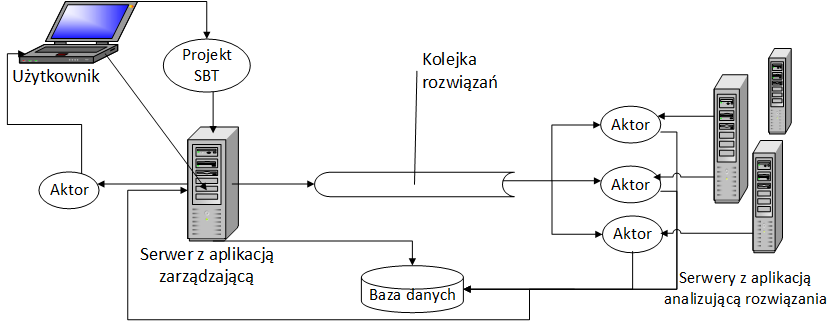
\includegraphics[width=1.05\hsize]{fig/scaxerciser_schemat}
\caption{Schemat komunikacji pomiędzy różnymi elementami systemu}
\source{Opracowanie własne}
\end{figure}

\section{Użyte technologie}

\subsection{Play Framework}

\subsection{AngularJS}

\subsubsection{Testy w AngularJS}

\subsection{MongoDB}

% zakończenie 
\summary
Możliwości, jakie stoją przed archiwum prac magisterskich opartych na
XML-u, są ograniczone jedynie czasem, jaki należy poświęcić na pełną
implementację systemu. Nie ma przeszkód technologicznych do stworzenia
co najmniej równie doskonałego repozytorium, jak ma to miejsce w
przypadku ETD. Jeżeli chcemy w pełni uczestniczyć w rozwoju nowej ery
informacji, musimy szczególną uwagę przykładać do odpowiedniej
klasyfikacji i archiwizacji danych. Sądzę, że język XML znacznie to
upraszcza.

% załączniki (opcjonalnie):
%\appendix
%\chapter{Tytuł załącznika jeden}

%Treść załącznika jeden.

%\chapter{Tytuł załącznika dwa}

%Treść załącznika dwa.

% wymuszenie pokazania bibliografii
\nocite{Hinojosa:2013:TIA}

% literatura (obowiązkowo):
\bibliographystyle{unsrt}
\bibliography{xml}

% spis tabel (jeżeli jest potrzebny):
\listoftables

% spis rysunków (jeżeli jest potrzebny):
\listoffigures

\oswiadczenie

\end{document}
